
\chapter{Label Propagation}
\label{ch:label-propagation}

Web browsers which execute JavaScript code allow pages to load JavaScript and HTML code from many different sources into the same execution context.
This work distinguishes between JavaScript programs by tagging each with a different label representing its domain of origin.
Many web pages using this technique contain cooperating functions which generate shared objects.
Each object created or modified via the confluence of separate scripts bears a label which tracks all domains influencing the object.

\begin{figure}[ht]
  \centerline{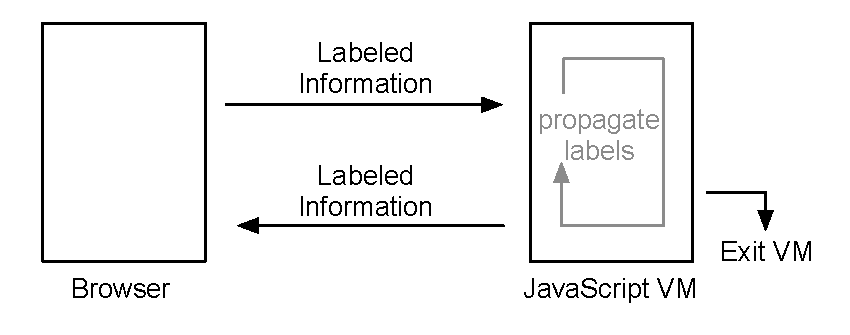
\includegraphics[keepaspectratio=true]{images/browserinteraction.pdf}}
  \caption{Interaction of the browser and the JavaScript~VM}
  \label{fig:browserinteraction}
\end{figure}

Figure~\ref{fig:browserinteraction} illustrates the interaction between the browser and the JavaScript engine.
Before the browser hands a script and its input data to the JavaScript VM, it first labels the script to indicate the domain of origin.
The VM then compiles the script source into an internal bytecode representation.
During this process, static analysis enables the instrumentation of additional bytecodes that allow information flow tracking during execution.

\section{Label Lattice}

This work takes inspiration from the decentralized label model~\cite{myers.liskov+00}.
Each web domain corresponds to a separate security principal, shown in the bottom row of Figure~\ref{fig:label-lattice}.
The information flow framework extends JavaScriptCore with a \code{LabelRegistry} which maps web domains to unique bit positions within the 64-bit label portion of a \code{JSValue}.
This configuration allows labels to represent any element within the lattice over web domains.
Figure~\ref{fig:label-lattice} depicts an example lattice for a page pulling JavaScript programs from three separate domains.

\tikzset{arrow/.style={
  decoration={markings,mark=at position 1 with {\arrow[scale=2.5]{latex'}}},
  postaction={decorate},
  shorten >= 0.4pt}
}

\tikzset{labarrow/.style={
  decoration={markings,
              mark=at position 0 with {\arrow[scale=1.5]{|};},
              mark=at position 1 with {\arrow[scale=2.5]{latex'};}
             },
  postaction={decorate},
  }
}

\tikzset{labelprop/.style={
  decoration={markings,mark=at position 1 with {\arrow[scale=2.5]{latex'}}},
  postaction={decorate},
  shorten >= 0.4pt}
}

\begin{figure}[ht]
\begin{tikzpicture}[node distance = 1cm, auto,
    force/.style={rectangle, inner sep=5pt, text badly centered, minimum height=.8cm}
    ]

    \begin{scope}[yshift=3.75cm, xshift=-7cm]
    \node[shape=rectangle, draw] {
       \begin{tabular}{l|c}
          \multicolumn{2}{c}{\code{LabelRegistry} mapping} \\
          \hline
          example.com & \texttt{0001} \\
          maps.com & \texttt{0010} \\
          ad.com & \texttt{0100} \\
       \end{tabular}
    };
    \end{scope}

    \begin{scope}
    \matrix[nodes={force}, column sep=1cm] {
        \node (ex) {example.com}; &
        \node (mp) {maps.com}; &
        \node (ad) {ad.com}; \\
    };
    \end{scope}

    \begin{scope}[yshift=2cm]
    \matrix[nodes={force}, column sep=.5cm] {
      \node (exUmp) {example.com $\sqcup$ maps.com}; &
      \node (exUad) {example.com $\sqcup$ ad.com}; &
      \node (mpUad) {maps.com $\sqcup$ ad.com}; \\
    };
    \end{scope}

    \begin{scope}[yshift=4cm]
    \matrix[nodes={force}, column sep=1cm] {
      \node (exUmpUad) {example.com $\sqcup$ maps.com $\sqcup$ ad.com}; \\
    };
    \end{scope}

    \draw[arrow] (ex) -- (exUmp);
    \draw[arrow] (ex) -- (exUad);

    \draw[arrow] (mp) -- (exUmp);
    \draw[arrow] (mp) -- (mpUad);

    \draw[arrow] (ad) -- (exUad);
    \draw[arrow] (ad) -- (mpUad);

    \draw[arrow] (exUmp) -- (exUmpUad);
    \draw[arrow] (exUad) -- (exUmpUad);
    \draw[arrow] (mpUad) -- (exUmpUad);

\end{tikzpicture}
  \caption{Interaction of the browser and the JavaScript~VM}
  \label{fig:label-lattice}
\end{figure}

Throughout execution, the modified JavaScript VM attaches the security labels to new JavaScript values based on the current execution context and web domain of origin.
Because labels can represent any element from the lattice, the interpreter is able to fully track which domains are involved in influencing each object.

\section{Label Operations}

The design decision to use a bit position encoding for web domains limits the framework to at most 64 domains.
Testing never encountered\footnote{Testing covered all pages within the \textit{Alexa Top 1000}~\cite{alexa}, but reloaded the browser for a clean slate between pages.} a single web page which included code from more than 64 different domains.
The framework contains no fundamental design flaws that would prevent an extension to the label encoding, if necessary.

\begin{definition}
  Given two security labels, $a$ and $b$, the {\bf join}, $a \sqcup b$, contains security principals that belong to the label $a$, the label $b$, or both.
\end{definition}

Using a bitwise representation allows the use of efficient bit arithmetic for computing the join (bitwise or) of two labels.
This operation occurs in every method call, assignment, and expression evaluation.
For example, when the program adds two numbers, the information flow framework labels the result with the join of the labels of the arguments and the label of the program counter.
Web applications today contain large amounts of JavaScript, which users expect to run without delay.
Label joining occurs frequently enough that any implementation other than bit arithmetic unacceptably penalizes the JavaScript runtime speed.

\begin{definition}
  Given two security labels, $a$ and $b$, the {\bf subsumes} relation, $a \sqsubseteq b$, is true if and only if the set of security principles comprising label $a$ is subset of the security principles comprising label $b$.
\end{definition}

The browser detects information leaks by comparing the label attached to a network request and the destination domain.
To assist with this task, labels support a subsumes relation that reveals the partial order of labels in the lattice.
If the label on the request contains principles other than the destination domain, the browser flags the request as a potential information leak.

\begin{definition}
  Given a security labels $a$ and $b$, the information flow VM {\bf upgrades} label $a$ with $b$ when it replaces $a$ with the join of $a$ and $b$, written $a \gets a \sqcup b$.
\end{definition}

When the Vm assigns value to an existing variable, it upgrades the label on the destination variable with the label attached to the source value.
Because assignment represents a mutation of memory, the VM also upgrades the destination label with the current pc-label.
The labels faithfully record the dependence of the assignment on the current security context.

%TODO: include equal relation?
%TODO: include strict subsumption?

\section{Control Flow Stack}
\label{sec:control-flow-stack}

In a dynamically typed language such as JavaScript, the techniques of static analysis that rely upon static typing (developed in languages such as Jif~\cite{jif}) are inapplicable.
As a result, the information flow modifications to the JavaScript VM perform tracking up to implicit active information flows.
By handing back label information on values used in construction of a network resource request, the VM modifications increase the data available to the browser for making network policy enforcement decisions 
However, to prevent information leak to third parties, the browser ultimately remains responsible for enforcing a security policy on network traffic.

The syntax of JavaScript programs allows for points where the control flow branches due to the evaluation of a runtime conditional.
At each of these points, the security context of any code executed within the token branch needs to reflect its dependence on the conditional.
To accomplish this task, we augment the JavaScript interpreter with a stack of labels, called the \term{control flow stack}.
As shown in Figure~\ref{fig:cf-stack}, the labels on this stack are in a 1-1 correspondence with the branches in control flow taken at runtime.
%This correspondence allows for tagging newly assigned values and function frames with the current security context.

\begin{figure}[ht]
  \centering
\begin{tikzpicture}[node distance = 0pt,
    box/.style={rectangle, draw, inner sep=3pt, text badly centered, minimum height=.8cm, minimum width=3cm},
    ]

%TODO: isn't there a split rectangle that I can use?

    \matrix[nodes={box}, anchor=south] (ops) {
      \node (condB) {conditional$_b$}; \\
      \node (condA) {conditional$_a$}; \\
      \node (func) {function call}; \\
      \node (dots) {\ldots}; \\
    };
    \node[below=of ops, align=center] {Operand and\\ Function Call\\ Stack};

    \matrix[nodes={box}, anchor=south, xshift=5cm] (labs) {
      \node (labFBA) {F $\sqcup$ C$_a$ $\sqcup$ C$_b$}; \\
      \node (labFA) {F $\sqcup$ C$_a$}; \\
      \node (labF) {F}; \\
      \node {\ldots}; \\
    };
    \node[below=of labs, align=center] {Control Flow\\ Stack};
    \node[right=of labFBA, align=left] {pc-label};

    \draw[labarrow] ($(condB.mid east)+(.1,0)$) -- (labFBA.mid west);
    \draw[labarrow] ($(condA.mid east)+(.1,0)$) -- (labFA.mid west);
    \draw[labarrow] ($(func.mid east)+(.1,0)$) -- (labF.mid west);
    %\draw[labarrow] ($(dots.south west)+(-.3,0)$) -- +(0,4);
    \draw[arrow] (condB.north) -- +(0,.8);
    \draw[arrow] (labFBA.north) -- +(0,.8);

\end{tikzpicture}
  \caption{Correspondence of branches in control flow and labels of the control flow stack.}
  \label{fig:cf-stack}
\end{figure}

The control flow stack records the runtime sequence of labels attached to the program counter.
At all time the top of the control flow stack holds the label of the current program counter, \term{pc-label}, identifying the security context of any operations currently under execution.
When the information flow VM assigns a value, it also joins the label attached to that value with the current pc-label.

\subsection{Monotonicity of Control Flow Stack}

We use two guidelines for maintaining the control flow stack:
\begin{enumerate}
 \item Whenever control flow diverges due to an \code{if}, \code{while}, \code{for}, \code{switch}, function call or similar statement, the VM duplicates the top of the control flow stack to indicate entry into a secure region.
 \item Whenever a control flow joins, the VM pops and discards the top of the control flow stack, restoring the pc-label to the value it had before the branch in control flow occurred.
\end{enumerate}

Of conspicuous absence in our guidelines (and the complete list of security bytecodes in Section~\ref{ch:security-bytecodes}) is an operation for pushing a specific security label onto the control flow stack.
According to the first guideline, the stack grows via successive duplications.
When the VM enters a secure code region it first duplicates the pc-label and then joins it with the label attached to the condition which cause the control flow branch.
This execution directly implies an important theoretical result:
\begin{theorem}
  At all times during program execution, the control flow stack contains monotonically increasing security labels.
\end{theorem}
\begin{proof}
 Let $i$ be the index of a label on the control flow stack, and $L_i$ be value of that label.
 Let the base of the stack be at index $i=0$.
 There are three basic operations which modify the control flow stack:
 \begin{enumerate}
  \item A \textit{pop} decreases the size of the stack, but does not modify any labels currently on the stack. Any existing relation between consecutive labels remains unchanged.
  \item A \textit{dup} duplicates the topmost label and pushes it onto the stack. This operation implies that all labels on the stack are of equal security, $L_i~=~L_{i+1}$.
  \item A \textit{join} upgrades the top of the stack by replacing it with the join of the top and an arbitrary label representing the control flow branch. This operation weakens the previous equality, $L_i~\sqsubseteq~L_{i+1}$.
 \end{enumerate}
 We now directly observe that for all indices $i$ on the stack, $L_i~\sqsubseteq~L_{i+1}$, which is the monotonicity condition to be proved.
\end{proof}

\section{Label Creep}
When the information flow VM assigns to a value, it upgrades the label attached to that value with the current pc-label (a.k.a. the top of the control flow stack).

The information flow VM system, explicitly labels values manufactured in a higher security context before allowing them to enter a lower security context, as may happen during via a function \code{return} statement.
The VM labels the result of computations involving two or more values using the join of the labels of all arguments.
The program counter acts as an implicit argument in all operations, so it's label too is joined in with the result.
As the interpreter executes, these joins steadily elevate the labels on objects within the system, a phenomenon known as \term{label creep}~\cite{sabelfeld.myers+03}.

At all times during program execution, a monotonically increasing list of security labels comprises the control flow stack.
All of the operations that our system performs on the control flow stack either leave the relationship between successive labels unchanged, or elevates the labels at the top of the stack.
Because all labels attached to values incorporate the current program counter label, which lies at the top of the control flow stack, it is important not to elevate the pc-label unless absolutely necessary.
Otherwise, an overly-conservative pc-label leads to the creation of values with unnecessarily elevated security labels.
This work therefore recognizes the monotonicity of the control flow stack to be the primary source of label creep.
